%\small Overview of the PLATO architecture. The pointer actor module processes local observations into agent and task embeddings, and then selects actions through three interconnected components: (1) Agent Encoding summarizes agent composition via mean, variance, minimum, and maximum statistics ($\mathbf{stats}$), embeds them with an MLP, and propagates temporal information through a memory LSTM to yield a recurrent query; (2) Task Encoding maps task features into the latent space, conditions them on the query through a key integrator, and organizes them into a sequence processed by an LSTM encoder; and (3) the Pointer Network combines the query with the encoded task sequence using additive attention to produce logits that define a distribution over available actions. The critic module evaluates the global state as a bipartite agent–task graph, where (1) a Graph Generator builds the graph structure, (2) a Node Encoder embeds agent and task features, (3) Graph Convolutional Layers capture relational dependencies, (4) Global Pooling aggregates node embeddings into a fixed-size representation, and (5) an MLP Head outputs the centralized value estimate.}



% \textbf{task encoding} (see \ref{taskencoding}), the observed tasks at time $t$, $\mathbf{o}^t_X$, are mapped into a hidden space conditioned on the aforementioned query. We do this per task through a \emph{key integrator} so that the key of each task is aware of the context of current agents and independent of other keys. 
%%producing a sequence for the pointer mechanism (see \ref{taskencoding}). 
% We combine each key with the query  through \textbf{the pointer decoder} to form an action distribution. The decoder attends over the key sequence with an additive attention mechanism that incorporates the query into each key independently, then normalizes the result.
%%The pointer head then attends over this task sequence with an additive attention mechanism that incorporates query and key into compatibility scores, ensuring each output logit reflects both task attributes and agent context. 

% These architectural elements make the pointer actor permutation invariant, scalable to unbounded sets of agents and tasks, adaptable as agents join or leave, and capable of producing valid action distributions over any number of tasks without retraining, padding, or index manipulation.

%%We use a pointer-network based actor (which we refer to as the pointer actor) that serves as the shared policy module in PLATO, enabling consistent behavior under agent openness where new or existing agents reuse the same parameters of the learned policy without retraining.
%In detail, the pointer actor preprocesses local observations (see \ref{obs_pre}) into two sets of features that serve as inputs for the subsequent encoding steps, using two novel designs: (a) \textit{agent encoding} (see \ref{agent_query}), where the present agents at time $t$ are summarized (see \ref{a_stats}) and passed through an MLP  to have an encoded summary, then we pass the encoded summery to LSTM to form a query (see \ref{eq:qt}), and (b) \textit{task encoding} (see \ref{taskencoding}), where the available tasks at time $t$ will later be mapped into a hidden space, conditioned on the query through a key integrator (see \ref{key_integrator}), and organized into a sequence for the pointer mechanism (see \ref{taskencoding}). The pointer head then attends over this sequence to produce the action distribution.

%%Several architectural choices ensure that the pointer actor is both permutation-invariant and scalable to unbounded set sizes. First, we compute summary \textbf{agent statistics} (mean, variance, minimum, and maximum) over the features of the current agent set to produce a fixed-length representation of the agent composition at time $t$ (see~\ref{a_stats}). This summary is inherently permutation-invariant and adapts seamlessly as agents join or leave the system. Second, we feed these statistics into a recurrent \textbf{LSTM} that produces the query vector. This recurrent query carries temporal context and smooths out abrupt changes, stabilizing the policy’s decisions over time even as agents appear or disappear (mitigating volatility when there is high agent churn; see \ref{agent_query}). Third, for each available task we generate a \textbf{task embedding} and then apply a \emph{key integrator} that adds the query vector to each task’s representation (see \ref{key_integrator}). This makes each task’s encoded key \emph{aware} of the current agents’ context, and it allows the pointer mechanism to flexibly handle any number of tasks without retraining (see \ref{taskencoding}). Finally, the \textbf{pointer head} uses an additive attention mechanism that directly incorporates the agent’s query when computing compatibility scores. In other words, the pointer head’s attention logits jointly reflect each task’s attributes and the current agent context. Because each output logit corresponds to one of the current tasks (or a no-op), the pointer actor can naturally produce a valid action distribution over an arbitrary number of tasks (with no need for padding or index trickery) and is invariant to any reordering of agents or tasks in the inputs.



%TODO Position free embeding
%MLP ENCODER
%ATTENTION DECODER
%POINTER + LSTM permutation invar break TODO
%Reasoning for single step decoding pointer head
%why no multi step

%\subsubsection{\textbf{Observation Preprocessor}}\label{obs_pre}
% This component separates agent and task features, enabling each encoder to handle its respective form of openness through specialized mechanisms.
% At each timestep $t$, the environment provides agents local observations $\mathbf{O^t}=\{o^t_i\}_{i=1}^{|N|}$. The preprocessor is a deterministic function that factors $\mathbf{O}$ into two tensors for encoding: agent features $\mathbf{o}_N^t$ and task features $\mathbf{o}^t_X$. This separation of agent and task features allows the pointer actor to handle each form of openness with a specialized encoding pipeline: one for the variable agent set and one for the variable task set.




% \subsubsection{\textbf{Agent Encoding (query path)}}\label{agent_query}
% Agent encoding receives agent features from the Observation Preprocessor (see~\ref{obs_pre}), aggregates them via Agent Statistics (see~\ref{a_stats}) to obtain a permutation-invariant summary of the current agent composition, maps this summary through an MLP to project it into the latent feature space, and updates it with an LSTM to produce a temporally smoothed recurrent query $q^t$ (see Eq~\ref{eq:qt}). This query captures both the current composition and its temporal context, and is shared with the Key Integrator in Task Encoding (see~\ref{key_integrator},~\ref{taskencoding}) and the attention mechanism in the Pointer Head (see~\ref{pointer_head}) to ensure consistent agent-aware decision-making across modules.


% %Agent encoding produces a recurrent query from the current agent set by summarizing composition with set-level statistics and updating it over time with an LSTM.

% \paragraph{\textbf{Agent Statistics.}}\label{a_stats}
% To address agent openness, this component summarizes the current agent set through a novel design that computes element-wise statistics (mean, variance, minimum, maximum) over agent features. The result is a fixed-length, permutation-invariant summary of agent composition. At time $t$, the agent composition is approximated by applying  statistical functions on $\mathbf{o}^t_n$:
% \begin{equation}
% d^t
%   = \big[\;\mu(\mathbf{o}^t_N),\;\sigma^2(\mathbf{o}^t_N),\;\min(\mathbf{o}^t_N),\;\max(\mathbf{o}^t_N)\;\big], \label{eq:agent-stats}
% \end{equation}
% where $\mu$ (mean), $\sigma^2$ (variance), $\min$ (minimum), and $\max$ (maximum) are statistical functions applied across agents.  
% $d^t$, is a size-agnostic, permutation-invariant signature of agent composition at time $t$. Using multiple statistics (instead of just a mean or sum) reduces the risk of aliasing different distributions of agent features into the same summary (for example, two very different sets of agents could share the same average feature vector). We then project $d^t$ through a feedforward network (MLP) to obtain an encoded summary $e^t_N = \mathrm{MLP}_s(d^t)$.

% These statistics form the \emph{query} for our pointer network later. We create the query by encoding the Statistics with a multilayer perceptron (MLP)~\cite{rumelhart1986learning_mlp}. Then, we use a long-short term memory module \cite{lstm} to smooth our query over time,
% \begin{equation}\label{eq:qt}
% q^t = \mathrm{LSTM} \left (\mathrm{MLP}_s \left (d^t \right ), q^{t-1} \right ).
% \end{equation}

% \noindent\textit{where} \(q^t\) is the recurrent query at time \(t\);
% \(q^{t-1}\) is the previous query;
% \(\mathrm{MLP}_s(\cdot)\) is a feedforward encoder for the agent statistics \(d^t\);
% and \(\mathrm{LSTM}(\cdot)\) updates the query using the current encoded input and past hidden state.



% In effect, $q^t$ summarizes the agent set at time $t$ while incorporating knowledge of past compositions through the LSTM state $q^{t-1}$. This temporal smoothing is important for stable policy behavior: when the agent set changes unpredictably from $t-1$ to $t$ (due to agents arriving or departing), the LSTM’s memory helps $q^t$ adapt smoothly rather than changing erratically. Because the LSTM processes only the summary $e^t_N$ (which does not depend on any ordering of agents), the query $q^t$ is insensitive to the permutation of agents in $\mathbf{o}_N^t$. In other words, agent encoding produces a query that is both representative of the current agent set and consistent over time, without being tied to any particular ordering of agents.

%TODO Old content replaced by above
%where $\mathrm{MLP}_a$ is a feedforward encoder that maps the statistics vector $\mathbf{a}_s$ into a latent representation  $\mathbf{e}_s $.  
%This yields explicit \emph{awareness of the agent composition} at each step, and because the statistics depend on \textit{feature statistics rather than identities}, \emph{previously unseen agents with similar features can be captured at execution time} without retraining.

%TODO, need a distinctive name.
%\paragraph{\textbf{LSTM}}\label{agent_lstm}
%This component encodes the agent statistics with an LSTM to produce a temporally smoothed query that carries forward agents context, ensuring stable adaptation as agents enter or exit under openness. Specifically, the latent representation $\mathbf{e}_s$ is passed to an LSTM~\cite{lstm} unit:
% \begin{equation}
% \mathbf{h}_s = \mathrm{LSTM}_{\mathrm{a}}(\mathbf{e}_s),
% \end{equation}
% where $\mathrm{LSTM}_{\mathrm{a}}$ is a recurrent encoder that preserves temporal memory across timesteps. Its hidden state $\mathbf{h}_s$ serves as the recurrent \emph{query}. Encoding the agent statistics with an LSTM yields a temporally smoothed query that carries forward agents context, enabling stable adaptation under AO and TO.

%\paragraph{\textbf{Permutation Invariant Query.}}
%The LSTM maintains permutation invariance with respect to agent ordering while providing temporal consistency across timesteps. Because $\mathbf{e}_s$ is derived from permutation-invariant statistics (mean, variance, minimum, maximum) over the agent set, any reordering of agents in $\mathbf{o}_t^{(a)}$ yields identical input to the LSTM. The recurrent encoder processes a \emph{temporal sequence of composition summaries} rather than a spatial sequence of individual agents, thus preserving permutation invariance in the agent dimension while capturing temporal dependencies in the time dimension. This design ensures that the query $\mathbf{h}_s$ adapts smoothly to dynamic changes in agents composition—agents can join or leave in any order without affecting the learned representation—while the LSTM's hidden state carries forward historical context to stabilize decision-making under rapid agent churn.
 %because these statistics summarize the entire agent set, the query representation adapts smoothly as agents join or leave, enabling stable decision-making under agent openness (AO).   

%**************************************

% \subsubsection{\textbf{Task Encoding (key path)}} \label{taskencoding}

% This component encodes the current set of available tasks into latent key representations for attention-based action selection. It receives raw task features from the Observation Preprocessor (see~\ref{obs_pre}) and projects them through an MLP to obtain task embeddings. These embeddings are then conditioned on the agent’s recurrent query (see~\ref{agent_query}) via the key integrator (see~\ref{key_integrator}), producing agent-aware task keys that reflect both task attributes and agent context. The resulting integrated keys $\mathbf{k}^t$ are passed to the pointer head (see~\ref{pointer_head}), where attention computes the final action distribution over the dynamic task set.

%%The task encoding module maps raw task observations into key vectors that are compared against the agent query (see~\ref{agent_query}), enabling attention to select among variable task sets in a agent composition-aware manner.

% \paragraph{Task Encoder.}\label{task_encoder} 
% This component maps each raw task observation into a latent key embedding through an MLP, producing task representations that capture essential task attributes while remaining compatible with variable task set sizes.
% \begin{equation}
% k^{t_x} = \mathrm{MLP}_k(o^t_x), \label{eq:task-mlp}
% \end{equation}
% \noindent\textit{where} \(k^{t_x}\) is the latent key embedding for task \(x\) at time \(t\);
% \(o^t_x \in \mathbf{o}^t_X\) is the raw feature vector of task \(x\);
% \(\mathrm{MLP}_k(\cdot)\) is a feedforward encoder that maps task features to the latent space;
% and \(\mathbf{k}^t = [k^{t_1}, \ldots, k^{t_{|\mathbf{o}^t_X|}}]\) is the collection of all encoded task keys.
% We consider no-op actions through a learnable embedding projected through the same MLP and appended to $\mathbf{k}^t$.  
% This full vector of keys, $\mathbf{K}^t$, is:
% \begin{equation}
% \mathbf{K}^t = [k^t_1; \dots; k^t_{|\mathbf{o}^t_X|}; k^t_{\textsc{NOOP}}]. \label{eq:task-stack}
% \end{equation}

% \paragraph{Key Integrator.}\label{key_integrator} 

% This component conditions each task embedding on the current agents context (see~\ref{agent_query}) by integrating the agent query into task keys, yielding agent-aware representations for attention-based selection.
%%In attention, each item $i$ is represented by a \emph{key} vector $\mathbf{k}_i$ that is compared to a \emph{query} $\mathbf{q}$; a compatibility score (e.g., $u_i=\mathbf{v}^\top\tanh(\mathbf{W}_k\mathbf{k}_i+\mathbf{W}_q\mathbf{q})$) determines how much the model should focus on item $i$. In PLATO, keys are the encoded task representations that the agent’s query attends over to select an action.

% In attention mechanisms, generally, each candidate (here, a task) is represented by a \emph{key}, which interacts with a \emph{query} to compute attention scores for selection. To inject the agents' context, $q^t$, into every available task to obtain an agent-aware selection, we adopt a key-integration operation inspired by modulation-based feature fusion (e.g., FiLM \cite{perez2018film}):  
% \begin{equation}\label{eq:key-integrator-eq}
% e^t_{K,x} = \mathrm{MLP}(k^t_x + \mathbf{W}_c \times q^t), \qquad 
% \mathbf{e}^t_K = [e^t_1; \dots; e^t_{|\mathbf{o}^t_X|}; e^t_{\textsc{NOOP}}]
% \end{equation}

%% redundant.
%%Shifting task keys by the agent query makes them agent-aware, so our design of the attention scores reflects both task attributes and the current agents while preserving permutation invariance.  

%% do we need this? -NOPE
%%This operation applies the query to all available tasks in $O(|\mathbf{o}_t^{(t)}|)$ time, avoiding the $\mathcal{O}(|\mathbf{o}^t_N|\cdot|\mathbf{o}^t_X|)$ cost of explicit agent–task pairings, while preserving permutation invariance.
% \noindent\textit{where} \(e^t_{K,x}\) is the integrated key embedding for task \(x\);
% \(k^t_x\) is the encoded task key from Eq.~\eqref{eq:task-mlp};
% \(\mathbf{W}_c\) is a learnable projection matrix aligning the query dimension with task embeddings;
% \(q^t\) is the recurrent agent query from Eq.~\eqref{eq:qt};
% \(\mathrm{MLP}(\cdot)\) is a feedforward layer that fuses task and query features;
% and \(\mathbf{e}^t_K\) is the full set of agent-aware task embeddings, including the no-op key \(e^t_{\textsc{NOOP}}\).


% Note that this agent-aware conditioning, to our knowledge, has not appeared in MARL or pointer-network policies. Prior MAPPO and transformer-based methods (e.g., \cite{mappo, foerster2018counterfactual_coma, dgn, gpl, dicg}) either concatenate or cross-attend embeddings, which requires fixed structures or masking and scales as $\mathcal{O}(|N|\cdot|X|)$. In contrast, our formulation injects the agent context into each task key through a shared linear projection, producing agent-aware task embeddings in $\mathcal{O}(|X|)$ time. This explicit conditioning simplifies attention learning and improves stability under openness.

%**************************************
%\subsubsection{\textbf{Pointer Decoder}}\label{pointer_head}
%This component is a modified pointer-network decoder that transforms the agent based query and task based keys into a stochastic policy conditioned on agent composition, enabling robust action selection under openness. It uses one-step attention \cite{attention} to decode $q^t,e^t_K\to \pi$. This differs from typical pointer networks \cite{ptr}, which use an LSTM in its decoder. Next we discuss, this and other decoder changes for openness.

%Unlike the original design, which relies on an LSTM decoder with sequential processing, our pointer network %employs an MLP encoder for task keys and 
%
% by architectural modifications for openness, and consists of three key components that transform  keys $\mathbf{K}^t$ into actionable policies, as summarized below.


%\paragraph{\textbf{MLP Encoder}}\label{pointer_encoder}
%Instead of using a conventional decoder to attend over the input sequence and the hidden representation for each input element (as generated by the LSTM-based encoder), we employ an MLP encoder to ensure both \emph{permutation invariance} and \emph{position-free embeddings}. Conventional pointer networks that use LSTM decoders introduce position-dependent biases because they process tasks sequentially. The encoder processes each integrated key independently:
%\begin{equation}
%\mathbf{E}_{k,i} = \mathrm{MLP}_{\mathrm{enc}}(\mathbf{sk}_{t,i}), \quad i = 1, \ldots, |\mathbf{o}_t^{(t)}| + 1
%\end{equation}
%This position-free encoding is crucial for openness because it allows the network to reason about task relationships regardless of task ordering or set size. Tasks may have intrinsic properties that influence selection priority, and the MLP captures these features without imposing artificial sequential dependencies. By avoiding recurrent architectures at this stage, we ensure that reordering tasks in $\mathbf{sk}_t$ does not affect their learned representations.


%\paragraph{\textbf{Attention Mechanism}}


%In conventional pointer networks, the decoder is an LSTM that maintains a hidden state across steps, while attention computes compatibility scores between the decoder state (query) and the encoder outputs (keys). These scores are normalized to obtain a distribution over key positions with a support $|\text{keys}|$. 
%therefore, the attention weights themselves constitute the output rather than a fixed vocabulary. 
%TO requires us to select \emph{one task per timestep} rather than an ordered sequence (as in TSP \cite{flood1956traveling}). We already model temporal continuity in the agent encoder's LSTM (see Section~\ref{agent_query}). Requiring only one task position allows us to replace the sequential decoder with a one-step attention mechanism, which treats keys independently. This avoids position bias and better supports openness.  


%The critic (Section~\ref{critic}) constructs a bipartite agent–task graph from the global state, encodes agent and task nodes into a shared hidden space with lightweight MLPs, propagates relational information via two GCN layers with a residual connection, and aggregates by global mean pooling; a small pre-head MLP then feeds a single linear value head to produce the centralized state value.



%We present a Graph Neural Network (GNN)-based value critic for our system. Our approach leverages graph convolutions \cite{kipf2016semi} to capture relationships between agents and environmental elements (fires) in a unified representation space, enabling effective value function approximation in complex multi-agent scenarios.  This approach helps the pointer network policy to estimate the value of each open state of the environment.
%\begin{equation} \label{eq:gcn}
%\mathbf{H}^{(\ell)} = \text{ReLU}\!\left(\tilde{\mathbf{D}}^{-1/2} \tilde{\mathbf{A}} \tilde{\mathbf{D}}^{-1/2} \mathbf{H}^{(\ell-1)} \mathbf{W}^{(\ell)} \right),
%\end{equation}


%The centralized critic builds a bipartite agent–task graph (see \ref{global_graph}) from the global state (see Figure \ref{fig:global_graph}), encodes agent and task nodes with an MLP (see \ref{node_encoder}) into a shared hidden space, and propagates relational information through two GCN layers (see \ref{gcn}). We use mean pooling to aggregate node embeddings into a fixed-size representation. We pass this representation through an MLP and a final linear layer to produce the scalar state value (see \ref{critic_valuehead}). This GNN-based design \cite{kipf2016semi} captures agent-task interactions in openness, without padding or concatenation, enabling an effective value approximation in openness and providing reliable value estimates for the pointer network policy.


%We use two GCN layers to capture both direct (agent–task) and second-order (agent–task–agent/task–agent–task) interactions, while avoiding the over-smoothing issues that arise with deeper stacks. The encoded graph $\mathbf{e}_g$ is passed through two GCNs to propagate relational information among nodes. At layer $\ell$, the representation is updated as


% which is finally passed to a linear value head to estimate the state value:
% \begin{equation}
% V(s_t) = \mathbf{W}_v \mathbf{z} + b_v.
% \end{equation}

%eqref


% where . The per-update complexity is
% \begin{equation}
% M_{\mathrm{time}}^{\mathcal{L}_V}=
% \mathcal{O}\!\left(f_V \cdot (|\mathcal{N}|+|\mathcal{X}|) + |\mathcal{E}| \cdot f_V + |\mathcal{B}|\right).
% \end{equation}




%Both actor and critic parameters are optimized jointly using Adam~\cite{kingma2014adam},
%with gradient clipping and early stopping based on approximate KL divergence %\cite{kullback1997information} for stability.








%\paragraph{Convergence under Openness.}
%In conventional reinforcement learning, convergence is often determined by the stabilization of cumulative episode rewards.
%However, under openness, this criterion becomes unreliable: each episode may yield variable returns due to changing agent counts, task sets, and interaction dynamics. 
%We experimented with an alternative strategy based on monitoring policy parameter stability, i.e., measuring updates in $\theta$ or the magnitude of changes in gradients across episodes. 
%While this approaches provided a more reward-agnostic signal, it introduced two additional hyperparameters --- the magnitude threshold and the episode window size --- that proved difficult to tune reliably. 
%TODO number of episodes might change.
%For fairness and reproducibility, we therefore adopted a fixed training horizon of 500{,}000 episodes for PLATO and all baseline methods. Empirically, we observed that by this point learning curves stabilized across different configurations, providing a consistent and robust stopping criterion.




%\subsection{Training and Optimization} The model weights are initialized using orthogonal initialization with gain 0.5 to prevent the activation magnitudes from exploding as they flow through the network:
%\begin{equation}
%\initW \sim \text{Orthogonal}(0.5), \quad \initb \sim \mathcal{N}(0, 0)
%\end{equation}
%Layer normalization is applied after each encoder to stabilize learning:
%\begin{equation}
%\layernorm(\mathbf{x}) = \frac{\mathbf{x} - \mu}{\sigma} \odot \boldsymbol{\gamma} + \boldsymbol{\beta}
%\end{equation}
%where $\mu$ and $\sigma$ are computed across the feature dimension.
 %TODO hyper parameters for our solution
 %TODO Computing Hardware or setup
 %TODO PROofs & theorms
%\subsubsection{Critic Efficiency.} The critic runs in $\bigO(|\edgeset| \cdot d_h + |\nodeset| \cdot d_h^2)$ time and $\bigO(|\nodeset| \cdot d_h + |\edgeset|)$ space. We optimize memory via in-place operations, vectorized pooling.






%We employ Multi-Agent Proximal Policy Optimization (MAPPO) \cite{mappo} with Centralized Training and Decentralized Execution (CTDE) paradigm. 












%********************END of ACTOR%



%This design enables handling \emph{task openness} 
%natively: new tasks can be evaluated against the existing agents context without retraining, as attention operates in a learned feature space rather than fixed task indices.

%This should be shown as one piece later.
%In terms of complexity, the per-update time scales linearly with the number of available tasks $|\mathcal{X}|$, the policy hidden dimension, $f_\pi$, and $\mathcal{B}$:
%\begin{equation}
%M_{\mathrm{time}}^{\mathcal{L}_\pi}=\mathcal{O}\!\left(f_\pi \cdot |\mathcal{X}| + |\mathcal{B}|\right).
% \end{equation}

%and parameters are updated using the Adam optimizer \cite{kingma2014adam}.
%\subsubsection{Actor Loss} \label{actor_loss}
% \subsubsection{Critic Loss}\label{critic_loss}
%The centralized critic estimates $V_\phi(s_t)$ on the bipartite graph $\mathcal{G}^t=(\mathcal{N},\mathcal{X},\mathcal{E})$. The loss uses the PPO clipped value formulation~\cite{ppo}:%. We  describe PLATO in detail,  with the \textit{shared pointer-network actor} in Section~\ref{actor}, and the \textit{centralized GNN critic} in Section~\ref{crit}ic. 
% Finally, Algorithm~\ref{alg:plato} presents the .

%PLATO integrates pointer networks \cite{ptr} as shared actors with graph neural networks \cite{gnn} as centralized critics, trained jointly within a multi-agent proximal policy optimization framework \cite{mappo}. 


%\subsection{Differentiability}\label{sec:differentiability}
%MAPPO is a policy gradient method, it requires a differentiable policy and critic network. PLATO is differentiable with respect to its parameters $\theta$, $\phi$, and the learned no-op vector NO-OP.




%\textit{Proof.}   
%Each component of PLATO is a composition of differentiable and (subdifferentiable functions. The statistical functions in Eq.~\eqref{eq:agent-stats} (mean, variance, min, max) are piecewise-linear or smooth and admit subgradients. Each MLP consists of affine maps and ReLU or $\tanh$ activations, and are differentiable everywhere.  
%(iii) The LSTM in Eq.~\eqref{eq:qt} uses smooth gates (sigmoid, $\tanh$) and is fully differentiable.  
%(iv) The attention mechanism in Eq.~\eqref{eq:attention} is composed of affine projections, $\tanh$, and inner products, all differentiable.  
%(v) The softmax in  the policy output is smooth; gradients are computed through $\nabla_\theta \log \pi_\theta$ using PPO (see \ref{actor_loss}, \ref{critic_loss}), avoiding non-differentiable sampling.  
%(vi) The GCN update in Eq.~\eqref{eq:gcn} is an affine transformation followed by ReLU, hence piecewise-linear and differentiable almost everywhere.  
%(vii) Mean pooling and residual additions are linear and preserve differentiability.

%By closure of (sub)differentiability under composition, the overall mapping from inputs to policy logits and state values is differentiable almost everywhere.  


+

\subsection{Training}


We train the model end-to-end using MAPPO ~\cite{mappo} under CTDE (see Algorithm \ref{alg:plato}). The policy is parameterized by $\theta$ and the centralized critic by $\phi$. During training, agents collect trajectories through interaction with the environment. The pointer actor is updated via the clipped PPO objective,
\begin{equation}
\mathcal{L}_{\pi_i} =
\frac{1}{|\mathcal{B}|}\sum_{j \in \mathcal{B}}
\min\!\left(r_j^i\,\hat{A}_j,\;
\mathrm{clip}\!\left(r_j^i,\,1-\epsilon,\,1+\epsilon\right)\hat{A}_j\right)
- \beta_H\, H(\pi_\theta),
\end{equation}
where
\begin{equation}
r_j^i=\exp\!\big(\log \pi_\theta(a_j|s_j)-\log \pi_{\theta^{\mathrm{old}}}(a_j|s_j)\big).
\end{equation}
Here $\hat{A}_j$ is the generalized advantage estimate \cite{gae}, $\epsilon$ is the clipping threshold, and $\beta_H$ weights the policy entropy $H(\pi_\theta)$, controlling exploration. Our loss is  an average over mini-batches, $\mathcal{B}$. 

The critic estimates $V_\phi(s_t)$ from the global graph. We use MSE, with the PPO clipped value formulation~\cite{ppo}: 

\begin{equation}
\mathcal{L}_V=
\frac{1}{2|\mathcal{B}|}\sum_{j \in \mathcal{B}}
\max\!\left(\left(V_\phi^j-\hat{R}_j\right)^2,\;
\left(V_\phi^{\mathrm{clip},j}-\hat{R}_j\right)^2\right),
\end{equation}
where $V^{clip}$ is the PPO clipped formulation of MSE \cite{ppo}, $\hat{R}_j$ is the empirical return from GAE and $\epsilon_V$ is the value clipping threshold. $V^{clip}$ is calculated as,
\begin{equation}
V_\phi^{\mathrm{clip},j}=V_\phi^{\mathrm{old},j}+\mathrm{clip}\!\left(V_\phi^j-V_\phi^{\mathrm{old},j},-\epsilon_V,\epsilon_V\right).
\end{equation}

\begin{equation}\label{eq:key-integrator-eq}
k^t_x = \mathrm{MLP}_k\left (\mathrm{MLP}_x(o^t_x) + \mathbf{W}_c \times q^t \right ), \quad 
\mathbf{K}^t = [k^t_1 \dots k^t_{|\mathbf{o}^t_X|}; k^t_{\textsc{NOOP}}].
\end{equation}
The outer $\textsc{MLP}_k$, is part of the \emph{key integrator} and projects the conditioned \emph{key} to the decoder's hidden dimension.

The key integrator conditions each task key on $q^t$ (Eq.~\eqref{eq:key-integrator-eq}), making task selection explicitly dependent on the current agent composition under churn.

We create the \emph{key}, $k^t_x$, for a task, $x$, by embedding $o^t_x$ into a latent space using a $\mathrm{MLP}_x$. Then we use a \emph{key-integration} technique inspired by modulation-based feature fusion \cite{perez2018film} to condition each \emph{key} on the \emph{query}, 



\subsection{GNN Critic} \label{critic}

The centralized critic estimates the state value $V_\phi(\text{State}^t)$ under CTDE.
To represent $\text{State}^t$ when the numbers of agents and tasks vary over time, we construct a \textbf{global bipartite graph} $\mathcal{G}^t$ (Fig.~\ref{fig:global_graph}).
The graph contains two node types: agent nodes and task nodes.
We use a bipartite structure because agent entities and task entities have different semantics and feature spaces, and the only relations required for value estimation in our domains are \emph{agent--task feasibility} relations.


\[
\mathcal{G}^t = (\mathcal{X}, \mathcal{N}, \mathcal{E
}),
\]
which encodes the state, $\text{State}^t$, at time $t$, where 
\begin{itemize}
\item $\mathcal{X}^t \in \mathbb{R}^{|X|^t\times f_X}$ are \emph{task nodes} and contain $f_X$ many features, describing each task at time $t$.
\item $\mathcal{N}^t \in \mathbb{R}^{|N|^t\times f_N}$ are \emph{agent nodes} and contain $f_N$ many features, describing each agent at time $t$. 
%\item $\mathcal{V} = \mathcal{A} \cup \mathcal{T}$ contains agent nodes and task nodes,  
\item $\mathcal{E}$ includes undirected edges between all agent-task pairs which have an action, $\{\langle n,x\rangle | n\in \mathcal{N} \text{ and }x\in \mathcal{X}\}$.  
%\item $\mathbf{X} \in \mathbb{R}^{|\mathcal{V}| \times d_x}$ holds the initial node features derived from agent observations and task attributes.  
\end{itemize}

\begin{figure}
  \centering
  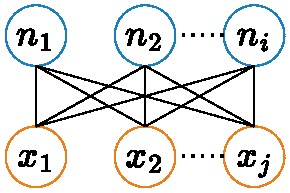
\includegraphics[width=0.6\linewidth]{figs/graph_revised.pdf}
\caption{\small This global graph represents the environment state for $i$ agents and $j$ tasks.
Edges encode agents ability to act on tasks.}
\label{fig:global_graph}
\end{figure}

We build a critic network on a graph convolutional neural network (GCN) \cite{kipf2016semi} which propagates  information between nodes (agents and tasks) by \textbf{message passing}. Before we use a GCN, we employ \textbf{MLPs} to bring $\mathcal{X}^t$ and $\mathcal{N}^t$ into the same space,
\begin{equation}
\label{eq:node-embedding}
\mathbf{h}_0^t = \text{Concat}\left [\text{MLP}_{\mathcal{N}}\left ( \mathcal{N}^t \right ), \text{MLP}_\mathcal{X}\left(\mathcal{X}^t \right ) \right ]\quad \mathbf{h}^t_0\in\mathbb{R}^{|\mathcal{G}^t| f_h},
\end{equation}
where $\mathbf{h}_0$ is the embedding of all nodes in $\mathcal{G}^t$, and $f_h$ is the hidden dim. Now, with fixed size features, we perform message passing, 
\begin{equation}
    \label{eq:message-passing}
    \mathbf{h}_1 = \mathrm{ReLU}\left (\frac{\mathbf{h}_0 W_{l}}{\sqrt{|N| \cdot |X|}} \right ) + \mathbf{h}_0,
\end{equation}
where we add $\mathbf{h}_0$ back in as a residual. We use two layers  (replacing $h_0$ with $h_{l-1}$ for layer $l$) to allow information to propagate from agent to agent and task to task through the other.

We map this graph to a scalar value estimate through mean pooling over nodes and a MLP$_v$ over pooled features,
\begin{equation}
\label{eq:value-pooling}
V(\text{State}^t) = MLP_v\left ( \frac{1}{|\mathcal{X}|+|\mathcal{N}|} \sum_{i=1}^{|\mathcal{X}|+|\mathcal{N}|} h^t_{2,i} \right ).
\end{equation}

\begin{algorithm}
\caption{\textsc{PLATO}}
\label{alg:plato}
\scriptsize
\begin{algorithmic}[1]
\State \textbf{Inputs:} env $e$, horizon $T$, actor $\pi_\theta$, critic $V_\phi$, initial observation $\mathbf{O}^0$
\For{$t=1\ldots T$} 
  \State $a^t_i\sim \textsc{PointerActor}(\mathbf{O}^t; \theta) \quad \forall i \in N$
  \State $\mathbf{O}^t,\text{State}^t,r^t\gets e(\mathbf{a}^t)$
  \State $\hat V^t \gets \textsc{GNNCritic}(\text{State}^t;\phi)$;\; store $(\cdot)$
  \State  compute GAE $\hat A^t$;\; update $\theta$ by PPO-clip;\; update $\phi$ by MSE$(\hat V^t,\hat R^t)$
\EndFor
\Statex

\Procedure{\textsc{PointerActor}}{$\mathbf{O}^t$}
  \State $\mathbf{o}_n^t,\mathbf{o}_X^t\gets \textsc{Preprocessor}(\mathbf{O}^t)$ 
  \Comment{Agent Encoding}
  \State $\mathbf{s}^t\!\gets\![\mu,\sigma^2,\min,\max](\mathbf{o}^t_{N})$
  \State $q^t \gets \mathrm{LSTM}\left (\textsc{MLP}_s(d^t),q^{t-1} \right )$
  \Comment{Task Encoding}
  \State $\mathbf{K}^t \gets \mathrm{MLP}_k\left (\mathrm{MLP}_x(o) + \mathbf{W}_c \times q^t \right ) \quad \forall o \in o^t_X \cup \textsc{NO-OP}$
  \State $u_i\!\gets\!\mathbf{v}^\top\tanh(\mathbf{W}_k \times k^t_x+\mathbf{W}_q\times q^t) \quad \forall k_x^t \in \mathbf{K}^t$ 
  \Comment{Pointer Decoding}
  \State  \textbf{return} $\mathrm{Cat}(\mathrm{softmax}([u_i]))$
\EndProcedure
\Statex
\Procedure{\textsc{GNNCritic}}{$\text{State}_t$} 
  \State form $\mathcal{G}^t=\langle\mathcal{X}^t,\mathcal{N}^t,\mathcal{E}^t\rangle$
  \State $\mathbf{h}_0^t \gets \text{Concat}\left [\text{MLP}_{\mathcal{N}}\left ( \mathcal{N}^t \right ), \text{MLP}_\mathcal{X}\left(\mathcal{X}^t \right ) \right ]$
  \State $\mathbf{h}^t_l \gets \textsc{GCN}(\mathbf{h}_{l-1}, \mathcal{E}) \quad \text{for each layer }l$
  %\!\gets\!\mathrm{ReLU}(\tilde{\mathbf{D}}^{-\frac12}\tilde{\mathbf{A}}\tilde{\mathbf{D}}^{-\frac12}\mathrm{ReLU}(\tilde{\mathbf{D}}^{-\frac12}\tilde{\mathbf{A}}\tilde{\mathbf{D}}^{-\frac12}\mathbf{e}_g\mathbf{W}^{(1)})\mathbf{W}^{(2)})$
  \State $\mathbf{M}^{(L)}\!\gets\!\frac{1}{|\mathcal{V}|}\sum_i(\mathbf{H}^{(2)}+\mathbf{e}_g)_i$;\;
  \State \textbf{return} $V=\mathbf{W}_v\,\mathrm{MLP}_v(\mathbf{M}^{(L)})+b_v$
\EndProcedure
\end{algorithmic}
\end{algorithm}

